\section{Conclusions}

\begin{frame}{Deep Learning Efficiency}
Building an efficient deep learning ecosystem is not a single factor problem,  
involving at least \textbf{four significant areas of improvements}:

\begin{itemize}
    \item Models (e.g. designing resource-efficient models)
    \item Platforms (e.g. DL frameworks that supports quantization)
    \item Infrastructure (e.g. low precision hardware)
    \item Hardware (e.g. domain-specific accelerations) 
\end{itemize}% designed to support the emerging need, 
\end{frame}

\begin{frame}{Summary}
    This thesis studies those DL methodologies that will allow us to unlock new levels of efficiency, incorporating the unique nature of optical hardware. Those studies include:
    \begin{itemize}
        \item Noise-aware training and adaptive initialization
        \item Lower Precision Neural Networks
        \item Non-negative Neural Networks
        \item Training acceleration through Multiplicative Updates and Sing-preserving Optimization  
    \end{itemize}
\end{frame}

\begin{frame}{Funding, Publications \& Rewards}
\begin{itemize}
    \item Co-authored \textbf{42 papers}, including \textbf{17 journal articles} and attracting \textbf{over 850 citations}.
    \item \textbf{Young Researcher Excellence Award 2024} \textit{Nominated by the Faculty of Sciences of the Aristotle University of Thessaloniki} 
\end{itemize}
    During my Ph.D. I joined and received funding from 6 European and National Projects:
\begin{enumerate}
  \scriptsize{\item \textbf{HAETAE:} Heterogeneously Integrated Multi-Material Photonic
    Chiplets for Neuromorphic Transfer Learning AI Engines (Grant Agreement: 101194393)} 
  \item \scriptsize{\textbf{SYMPHONY:} Smart systems for environmental pollution detection
    and biogas production based on cloud-connected silicon photonic and
    microelectronic hyperspectral sensor (Grant Agreement: 101135523)}
  \item \scriptsize{\textbf{DeepLet:} Efficient and Trustworthy Deep Learning (Grant
    Agreement: 16762)}
  \item \scriptsize{\textbf{PlasmoniAC:} Energy- and size-efficient ultra-fast plasmonic circuits for
    neuromorphic computing architectures (Grant Agreement: 871391)}
  \item \scriptsize{\textbf{DeepLight:} Photonic Neuromorphic Hardware for Deep Learning
    Applications over Light-enabled Integrated Systems (Grant Agreement: 4233)}
  \item \scriptsize{\textbf{OpenDR:} Open Deep Learning Toolkit for Robotics (Grant
    Agreement: 871449)}
  % \item \textbf{DeepStream:} Semantic Annotation and Metadata Enrichment of Open Video
  %   Streams Using Deep Learning project (Action “Investment Plans of Innovation”
  %   of the Operational Program “Central Macedonia 2014-2020”)
  % \item \textbf{DeepFinance:} Εφαρμογή Τεχνολογιών Βαθιάς Μάθησης για Ευφυή Διαχείριση
  %   Χρηματοοικονομικών Χαρτοφυλακίων μέσω Σημασιολογικής Ανάλυσης Ροών
  %   Κοινωνικών Δικτύων
  \end{enumerate}
\end{frame}

% \begin{frame}{Publications}
%     \begin{itemize}
%         \item Co-authored\textbf{ 42 papers}
%         \item Including \textbf{17 journal articles}
%         \item Attracting \textbf{over 850 citations} (\href{https://scholar.google.com/citations?user=EyaKPkwAAAAJ&hl=en}{Google Scholar})
%         \item Received \textbf{Young Researcher Excellence Award} by Faculty of Sciences of the AUTH
%     \end{itemize}
% \end{frame}

% \begin{frame}{Photonic Integration}
%   \begin{center}
%   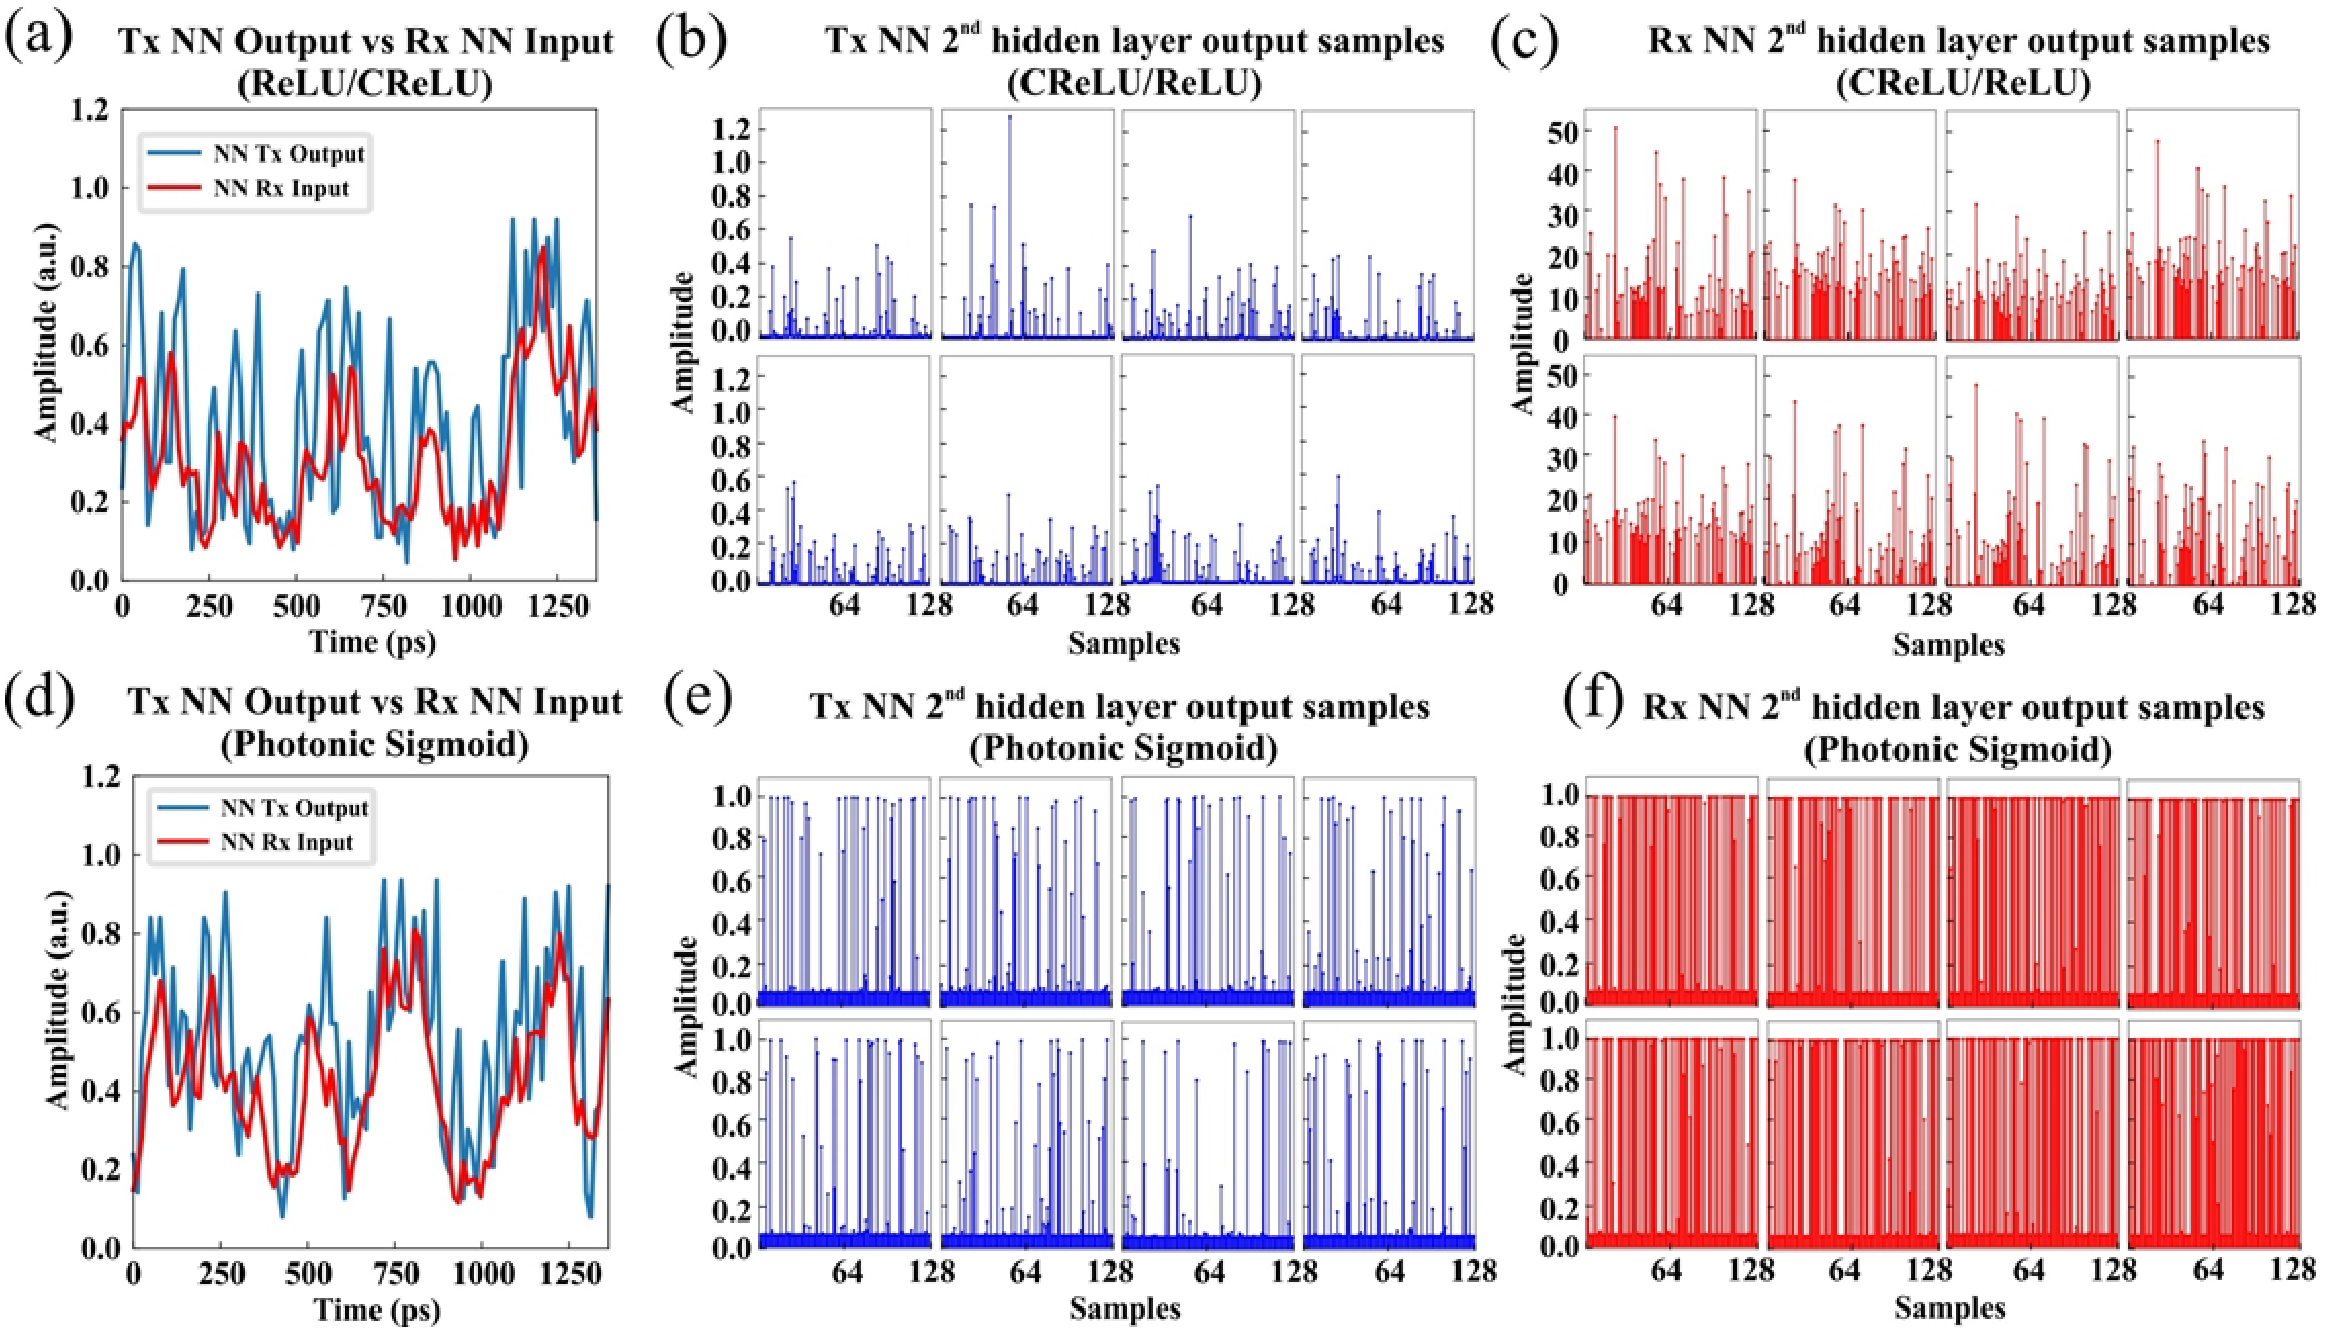
\includegraphics[width=0.5\linewidth]{sections/6_conclusions/images/experimental_analysis.jpeg}
%   \scriptsize{\textbf{\underline{Source:}} Roumpos, I., De Marinis, L., \textbf{Kirtas, M.}, Passalis, N., Tefas,
%       A., Contestabile, G., Pleros, N., Moralis-Pegios, M. and Vyrsokinos, K., 2023. \href{https://opg.optica.org/oe/fulltext.cfm?uri=oe-31-12-20068&id=531138}{High-performance end-to-end deep learning IM/DD link using optics-informed neural networks}. Optics Express}
%   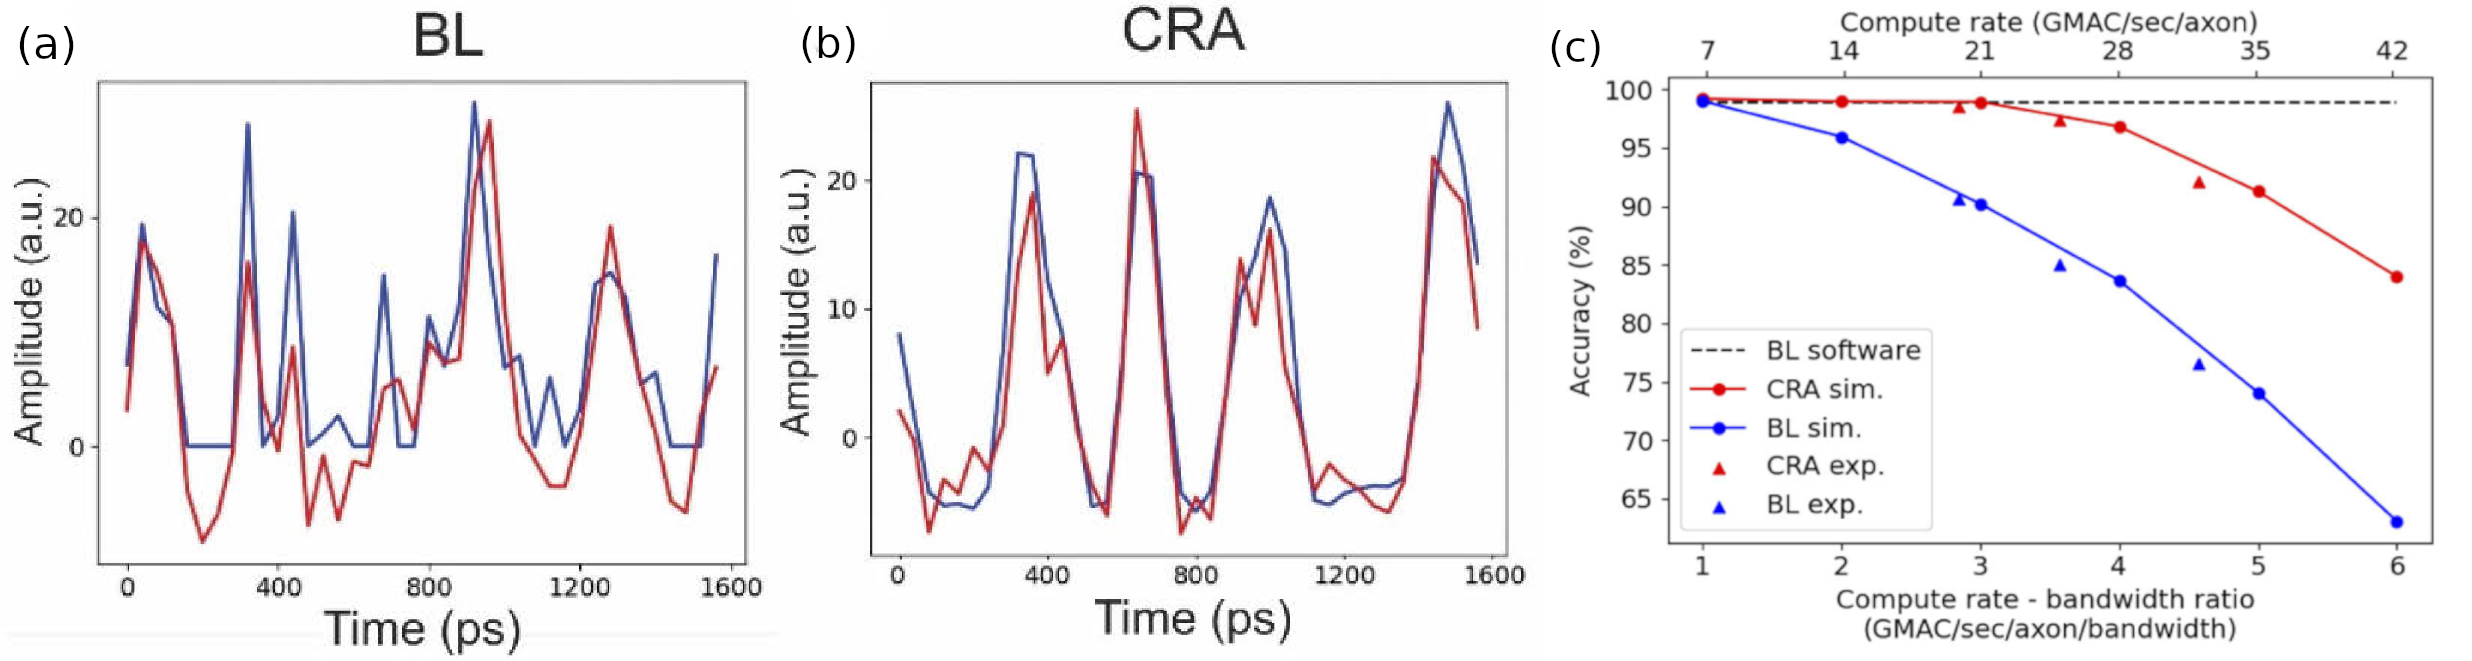
\includegraphics[width=\linewidth]{sections/6_conclusions/images/channel_overview.png}
%   \scriptsize{\textbf{\underline{Source:}} Mourgias-Alexandris, G., Moralis-Pegios, M., Tsakyridis, A., Passalis, N.,
%   \textbf{Kirtas, M.}, Tefas, A., Rutirawut, T., Gardes, F.Y. and Pleros, N., 2022. \href{https://opg.optica.org/oe/fulltext.cfm?uri=oe-30-7-10664&id=470426}{Channel response-aware photonic neural network accelerators for high-speed inference through bandwidth-limited optics.} Optics Express}
%   \end{center}
% \end{frame}

% \begin{frame}{Applications: Early DDoS Detection}
% \end{frame}

% \begin{frame}{Frame Title}
    
% \end{frame}